%
%	WISS 2015サンプルファイル (未来ビジョンテンプレート, 最後数行空き問題解決バージョン)
%
%	2010/07/12 Ver 1.0 秋田 純一
%	2010/08/04 Ver 1.1 後藤 真孝
% 	2011/09/27  Ver 1.4 渡邊 恵太 (協力:五十嵐悠紀)
% 	2015/02/08  Ver 1.5 大槻 麻衣
% 	2016/05/26  Ver 1.6 大槻 麻衣


\documentclass[a4paper,twoside,papersize]{wiss}

\usepackage{ascmac}
\usepackage[dvips]{graphicx}
\usepackage{nidanfloat} %% appended in WISS2010 for Future Vision (2010/7/7:akita)
\usepackage{multicol}
%\usepackage{color,array}
%\usepackage{boxedminipage}

%% balance.styを追加 (2012/9/27:watanabe, Igarashi)
\usepackage{balance}    %% 最後のページの高さを揃えるために追加  (2012/9/27:watanabe, Igarashi)
%%% 最後のページの2段組の高さを揃える.\balanceを入れる.
%%% そろえたくないときは,\nobalance

%% urlのOverflow対策
\usepackage{url}

\journalhead{わかるらんど: IoT時代の情報共有視覚化} %%%%%% ←← 著者において必ず記入すること

\begin{document}

\title{わかるらんど: IoT時代の情報共有視覚化}
\etitle{}%2012年では英文タイトルは廃止されました.記入しないでください.
%
%注意
%
%
% WISS2016かラシングルブラインドとなりました.投稿時に氏名と所属を記入してください.
\author{山田 尚昭\affil{慶應義塾大学大学院 政策・メディア研究科}  増井 俊之\affil{慶應義塾大学 環境情報学部}}

\begin{abstract}
全世界のセンサ情報やユーザの気分などを一覧表示したり
投稿したりできるシステム『\textsf{わかるらんど}』を提案する.
ニュースや天気予報のようなリアルタイム情報を並べて一覧表示する
「情報ダッシュボード」の利用が広まっているが,利用できる情報の種類は限られており,
ユーザが情報を投稿して共有することはできない.
『わかるらんど』は,単純で強力なWeb上の情報共有システム「WebLinda」上に構築された
汎用的な情報共有/視覚化システムであり,ユーザの気分を表明したり,
チャット文字列を投稿したり,センサ情報やWeb上の情報を表示したり,
ネット上のあらゆる情報を投稿/共有して一覧表示することできる.
『わかるらんど』の利用により,情報ダッシュボードとSNSやチャットシステムを
簡単に統合的に利用することができる.
本論文では,『わかるらんど』の思想及び利用経験について述べ,応用について考察する.
\end{abstract}

\maketitle

\section{はじめに}

WebやIoT機器などから発信されるフロー情報が巷にはあふれている。
フロー情報とはニュースや天気予報、SNSなどリアルタイムに常に流れていく情報のことである。

フロー情報を視覚化する手法として\textgt{ダッシュボード}(図\ref{dashing})がある。
ダッシュボードとは単一の画面に情報を並べて表示するもので、センサの値や株価などのフロー情報をひと目で把握するのに非常に便利である。
ダッシュボードには様々な製品やサービスが存在し、多くの組織で利用されている。
フロー情報のひとつである「人間の感情や現在の状況」というものをアウトプットする場としてテキストチャットやSNSが多くの人に利用されているが、
時間順に投稿をリストするタイムライン表示は投稿したものが流れていってしまったり投稿数の多い人ばかりが目立ってしまったりするという問題がある。

一般的にダッシュボードに表示される情報に加えて、人や環境の状態も単一の画面に表示する視覚化システム「わかるらんど」を提案する。

\begin{figure}[h]
\centering
\includegraphics[width=7cm]{images/dashing.eps}
\caption{ダッシュボード}
\label{dashing}
\end{figure}
\section{わかるらんど}
『わかるらんど』のユーザインタフェースは「ダッシュボード」と「投稿画面」の2つからなり,
画面右上のボタンで切り替えることができる.
図\ref{dashboard}はダッシュボードのスクリーンショットである.
ユーザが投稿したテキストやスタンプや,
各種のセンサのデータなどがリアルタイムに1つの画面に表示されている.
センサのデータなどは自動的に更新され,ユーザのリアクションは図\ref{console}の投稿画面で
ユーザ名を入力し,スタンプを一覧から選んで投稿することで
自分のアイコンの上にオーバーレイ表示される.
ユーザの投稿には表示時間が設定されており,
指定時間が経過すると自動的に投稿が取り下げられるため
いつまでも古い投稿が表示され続けてしまうということはない.

\begin{figure}[h]
\centering
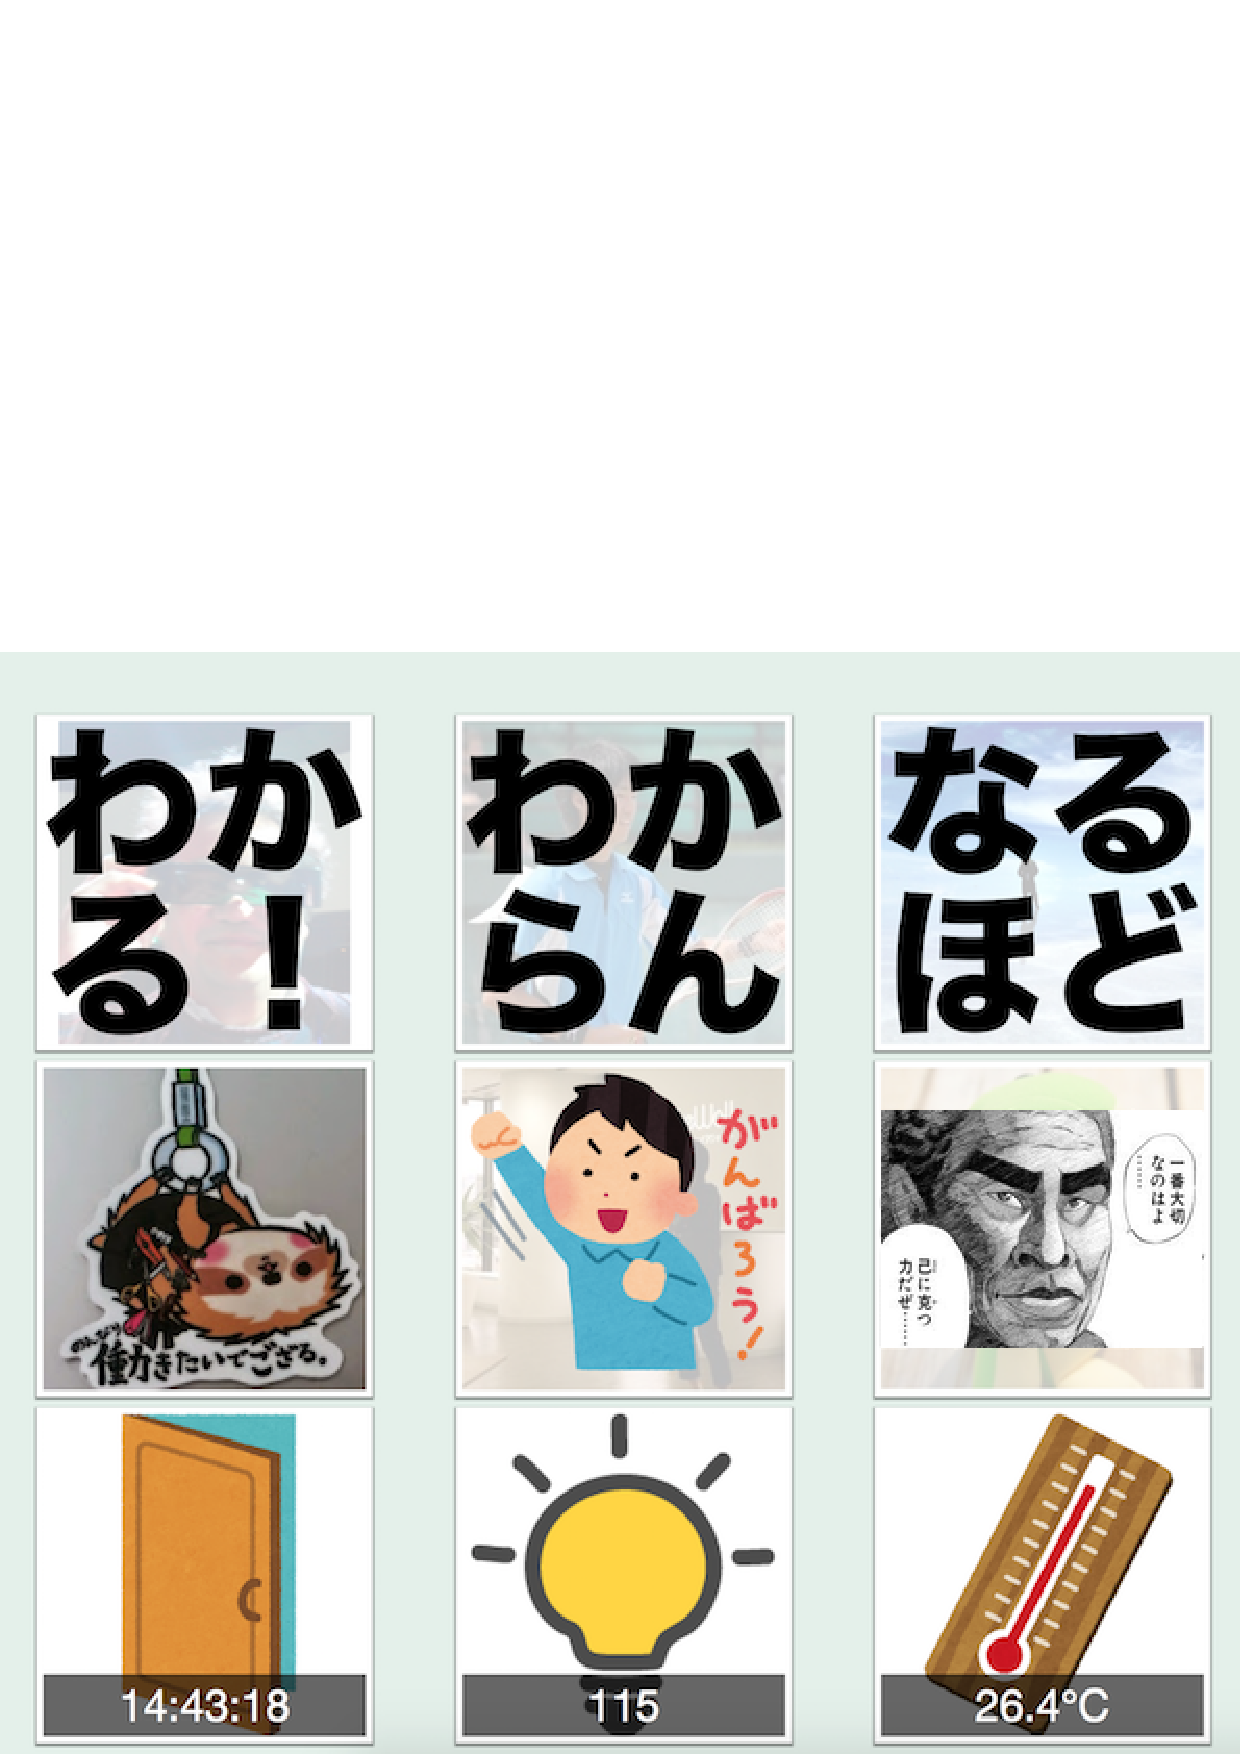
\includegraphics[width=6cm]{images/dashboard.png}
\caption{『わかるらんど』のダッシュボード}
\label{dashboard}
\end{figure}

\begin{figure}[h]
\centering
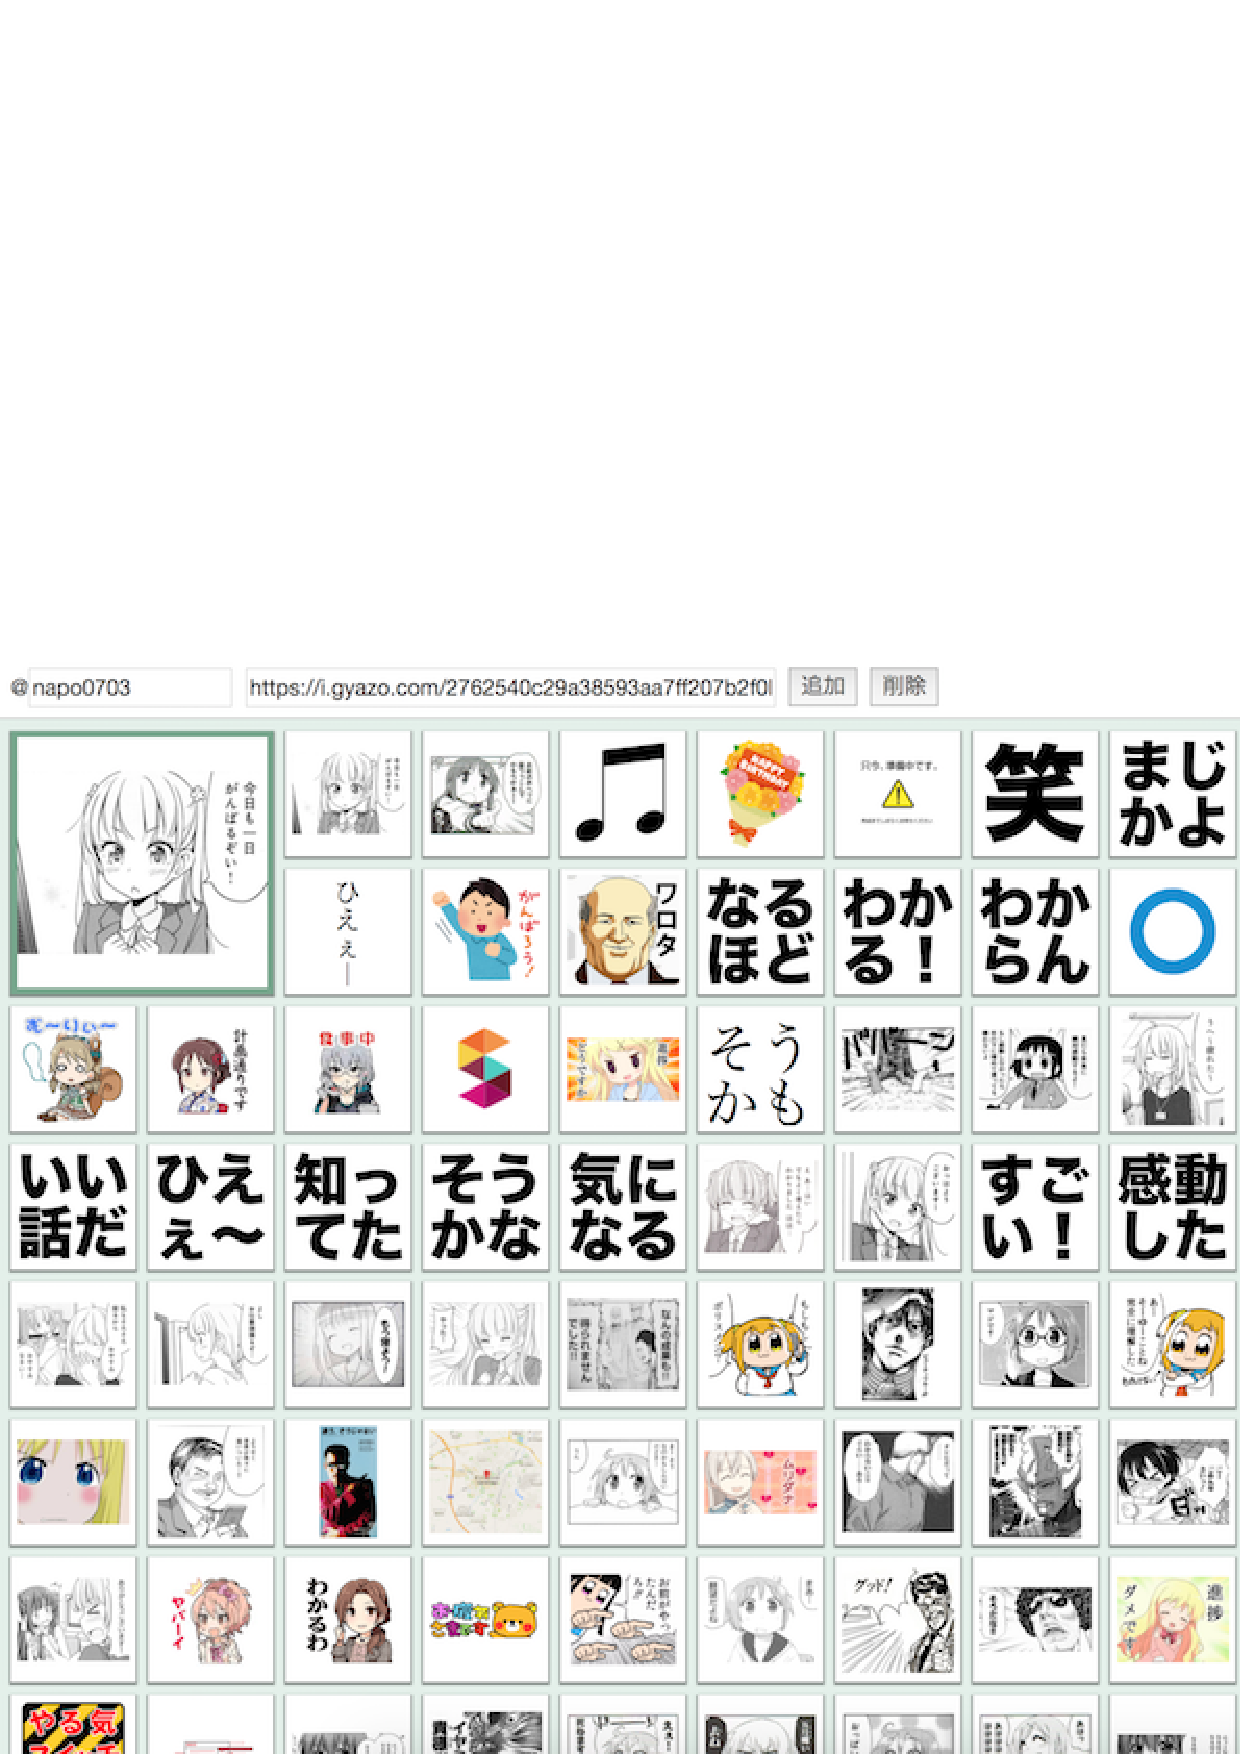
\includegraphics[width=6cm]{images/console.png}
\caption{『わかるらんど』の投稿画面}
\label{console}
\end{figure}
\section{実装}

『わかるらんど』のクライアントは\url{HTML/CSS/JavaScript}で実装されており,
通常のブラウザ上のWebアプリケーションとして動作する.
サーバは,並列計算プリミティブである
\textit{Linda}\cite{Carriero:1989:LC:63334.63337}を
Webサーバ上に実装した
\textit{WebLinda}\cite{shokai_furnitue}\footnote{https://github.com/node-linda/linda}
を用いて実装している.

\textit{WebLinda}は,橋本翔氏が開発したオープンソースソフトウェアで,
Node.jsの
WebSocketライブラリ「Socket.IO」で
実装されている.
\textit{WebLinda}は通常のWebサーバ上に実装されているため,
HTTP通信をサポートする様々な環境やプログラミング言語で利用可能である.
\section{議論}

\subsection{チャットシステムとしての利用}

LINE株式会社が提供するスマートフォン向けのコミュニケーションアプリである「LINE」は,日本で非常に多くの人に使われている.
LINEの基本機能はユーザが個人またはグループに対してテキストベースでメッセージを送信できるものであり,
従来のメッセンジャーアプリと機能の面で大きな違いがあるわけではない.
LINEの最大の特徴は「スタンプ」という大型の絵文字のようなピクトグラムを送信できることである.
スタンプはテキストで記述するのが難しい表現や感情を伝えるのに非常に適している.
また,一覧からスタンプを選ぶだけで送信ができるため,テキストを考えて入力するよりも速く簡単である.
近年ではメッセンジャーアプリだけではなくリアルタイムコミュニケーションが必要なオンラインゲームなどでもスタンプの利用が広まっている.

講義やコンファレンスではテキストチャットが利用されることが多いが,
発言にスタンプのみを用いるわかるらんどはチャットシステムが抱える問題を解決できると考える.
チャットシステムには3つの問題があると考える.

\begin{itemize}
\item 同時に多数が投稿するとすぐに流れていってしまう
\item 投稿数の多い人が目立ってしまう
\item 投稿しない人は全く投稿しない
\end{itemize}

チャットに限らず会議やコンファレンスなどでも特定の人だけが沢山発言し,発言しない人は全く発言しない状況はよくあることだ.
何かしらリアクションや発言をしたいが,気の利いたことを言わなければならない,的外れなことを言えないという環境が積極的な発言を妨げになっていると考える.
WISS2009のコミュニケーション支援システム「On Air Forum」の実証実験\cite{nishida2011}では1回以上発言した人が約半数であった.
思いつきを発言できる環境を作り1人でも多く参加する人を増やすことが,「多くの人の感情をひと目で把握したい」というわかるらんどの目的の達成に必要である.

わかるらんどは全員の最新の投稿のみを表示するインタフェースである,
スタンプしか投稿できず高度な意見を述べることは全く期待されないことから,

\begin{itemize}
\item 短時間に多くの人が投稿しても流れて見えなくなってしまうことがない
\item 投稿数が多いからといって目立つわけではない
\item 投稿のハードルが低い
\end{itemize}
というテキストチャットやタイムラインにはない特徴がある.

わかるらんどのインタフェースは長い文章を投稿するのに適していないのでわかるらんど上で議論を行うことは難しい.
発表の場合は最後に質問や議論の時間があるので議論はその時に行えばよい.
そもそも人が発表をしているときはチャットで議論なんてしてないで話を聞くべきである.

\subsection{実際の行動に基づく投稿}

別の作業を行っていてわかるらんどへの投稿をしたいときにブラウザを開いてスタンプを選んで押さなければならない.
前述のボタンやテンキーなど専用の入力装置も作ることができるが,投稿できるものが限られている.
自分が心のなかで「なるほど」と思ったらわかるらんどに「なるほど」と投稿したり,怒ったら怒っている絵文字を投稿したりしたい.
人間の実際の行動に基づいて,膝を打ったら「なるほど」,首を捻ったら「わからん」など慣用句と結びつけた投稿や,
髪をいじったら「考え中」など人の癖を利用した感情の推定も利用できるだろう.
\section{関連研究}

Information Dashboardは多くの製品やサービスが存在する。
研究としては、2つに区切られたレイアウトのDashboardのセルの配置を支援するものや、
ある課題の解決のためにどのような情報をダッシュボードに表示するべきかなどが議論されている。
Dashboardに人間の感情や現在の状況を表示するといった試みは今までに行われていないと思われる。
\section{結論}
人や環境の状態がリアルタイムにわかる視覚化システム「わかるらんど」を提案した.
非常に汎用で拡張性も高く,様々な場面での情報共有に利用されることが期待でき,
IoT時代の情報視覚化として広く利用されるとともに,
長い間続けられてきたテキストベースのコミュニケーションに終止符を打ち,
ピクトグラムベースのコミュニケーションの先駆け的存在となるだろう.

%%
%%	参考文献
%%
% \begin{thebibliography}{1}

% \bibitem{wiss} WISSホームページ.  http://www.wiss.org/.

% \bibitem{aoki1999} H.~Aoki, B.~Schiele, and A.~Pentland.  Realtime
% Personal Positioning System for Wearable Computers.  In
% \emph{Proceedings of the 3rd IEEE International Symposium on Wearable
% Computers}, pp. 37--43, 1999.

% \bibitem{rekimoto2000} 暦本 純一.  まえがき:WISS2000について.  インタラ
% クティブシステムとソフトウェアVIII, pp. i--ii. 近代科学社, 2000.

% \end{thebibliography}

\balance %最後の高さを揃えるために必要 (2012/9/27:watanabe, Igarashi)
\bibliographystyle{jwiss}
\bibliography{paper}

%%%%%%%%%%%%%%%%%%%%%%%%%%%%%%%%%%%%%%%%%%%%%%%%%%%%%%%%%%%%%%%%%%%%%
%%%%%%%%%%%%%%%%%%%%%%%%%%%%%%%%%%%%%%%%%%%%%%%%%%%%%%%%%%%%%%%%%%%%%
%% WISS2012では,「未来ビジョン」は以下のように,本文と同様の2段組形式で記載する.
%% 図を用いても良いが,枠のサイズ(縦93mm)を変更してはならない.
%% (WISS2010では,縦118mmでしたのでご注意下さい)

\begin{figure*}[!b]
\setlength{\unitlength}{1mm}\fboxrule=0.5pt

\vspace{-93mm} %% 未来ビジョンの枠が下がってしまうのを防ぐ WIS2012 カメラレディテンプレで追加  (2012/9/27:watanabe, Igarashi)

% 未来ビジョンの枠の描画
\begin{center}
\framebox[0.95\textwidth]{
\begin{minipage}{0mm}\begin{picture}(0,91)(0,0)\end{picture}\end{minipage}
}
\end{center}
\vspace*{-93mm}	% 未来ビジョンの枠の縦幅分だけ戻す

% 未来ビジョンの内容
\newbox\FUTURE
\setbox\FUTURE=\vbox{
\begin{minipage}[b]{0.9\textwidth}
\begin{multicols}{2}	% 二段組にする
\section*{未来ビジョン}
\setlength{\parindent}{10pt}	% 段落先頭の字下げ

% % % % % % % % % % % % % % % % % % % % % % % % % % % % % %
%	   未来ビジョンは,下記に記入して下さい		  %
% % % % % % % % % % % % % % % % % % % % % % % % % % % % % %

\vspace*{-1mm}

% フォントサイズ指定
\normalsize
%\large
%\small\setlength{\baselineskip}{12pt}
%\footnotesize\setlength{\baselineskip}{12pt}

わかるらんどは「人の気持ちを察したい」という思想から作られたシステムである.
初期のプロトタイプは文字が書かれた札を掲げるというアナログなものだった.
会議やコンファレンスなど多人数に向けての発表の場において最も悲しいことは,聴衆から何のフィードバックもないことである.
「わからん」「なるほど」といった簡単な相づちがあるだけでも印象は異なる.
私自身が口下手で感情のアウトプットが得意なほうではないこともあって,
思ったことを口にしやすいコミュニケーション環境をインタフェースの工夫によって作り上げることがこの研究のミッションである.
わかるらんどが私と同じ悩みを抱えている人の一助になれば幸いである.

%% 文章を補う図表を利用してもよい.
\vspace*{5mm}
\includegraphics[width=0.95\columnwidth]{images/wakaru.eps}
% % % % % % % % % % % % % % % % % % % % % % % % % % % % % %
%	   未来ビジョンは,上記に記入して下さい		  %
% % % % % % % % % % % % % % % % % % % % % % % % % % % % % %

\end{multicols}
\end{minipage}
}

% 未来ビジョンの内容の描画
\newlength{\FUTUREHT}
\setlength{\FUTUREHT}{\the\ht\FUTURE}	% 未来ビジョンの内容の縦幅保存
%\typeout{\the\wd\FUTURE}
%\typeout{\the\ht\FUTURE}
\hspace*{0.045\textwidth}	% 未来ビジョンの内容の横位置調整
\box\FUTURE
%\typeout{\the\FUTUREHT}
\vspace*{-\the\FUTUREHT}	% 未来ビジョンの内容の縦幅分だけ戻す
\vspace*{-10.9mm}		% 微調整

% 未来ビジョンの枠の領域の再確保(これがないと枠が下に沈み込む)
\begin{center}
\fboxrule=0pt
%\fboxrule=2pt	% デバッグ用: コメントアウトをやめて,同じ位置に枠が出るか?
\framebox[0.9\textwidth]{
\begin{minipage}{0mm}\begin{picture}(0,91)(0,0)\end{picture}\end{minipage}
}
\end{center}
\end{figure*}

%%%%%%%%%%%%%%%%%%%%%%%%%%%%%%%%%%%%%%%%%%%%%%%%%%%%%%%%%%%%%%%%%%%%%
%%%%%%%%%%%%%%%%%%%%%%%%%%%%%%%%%%%%%%%%%%%%%%%%%%%%%%%%%%%%%%%%%%%%%
\end{document}
